\subsection{Problema 4 - Modulação \texorpdfstring{$M$}{M}-PSK}

\begin{figure}[!ht]
    \centering
    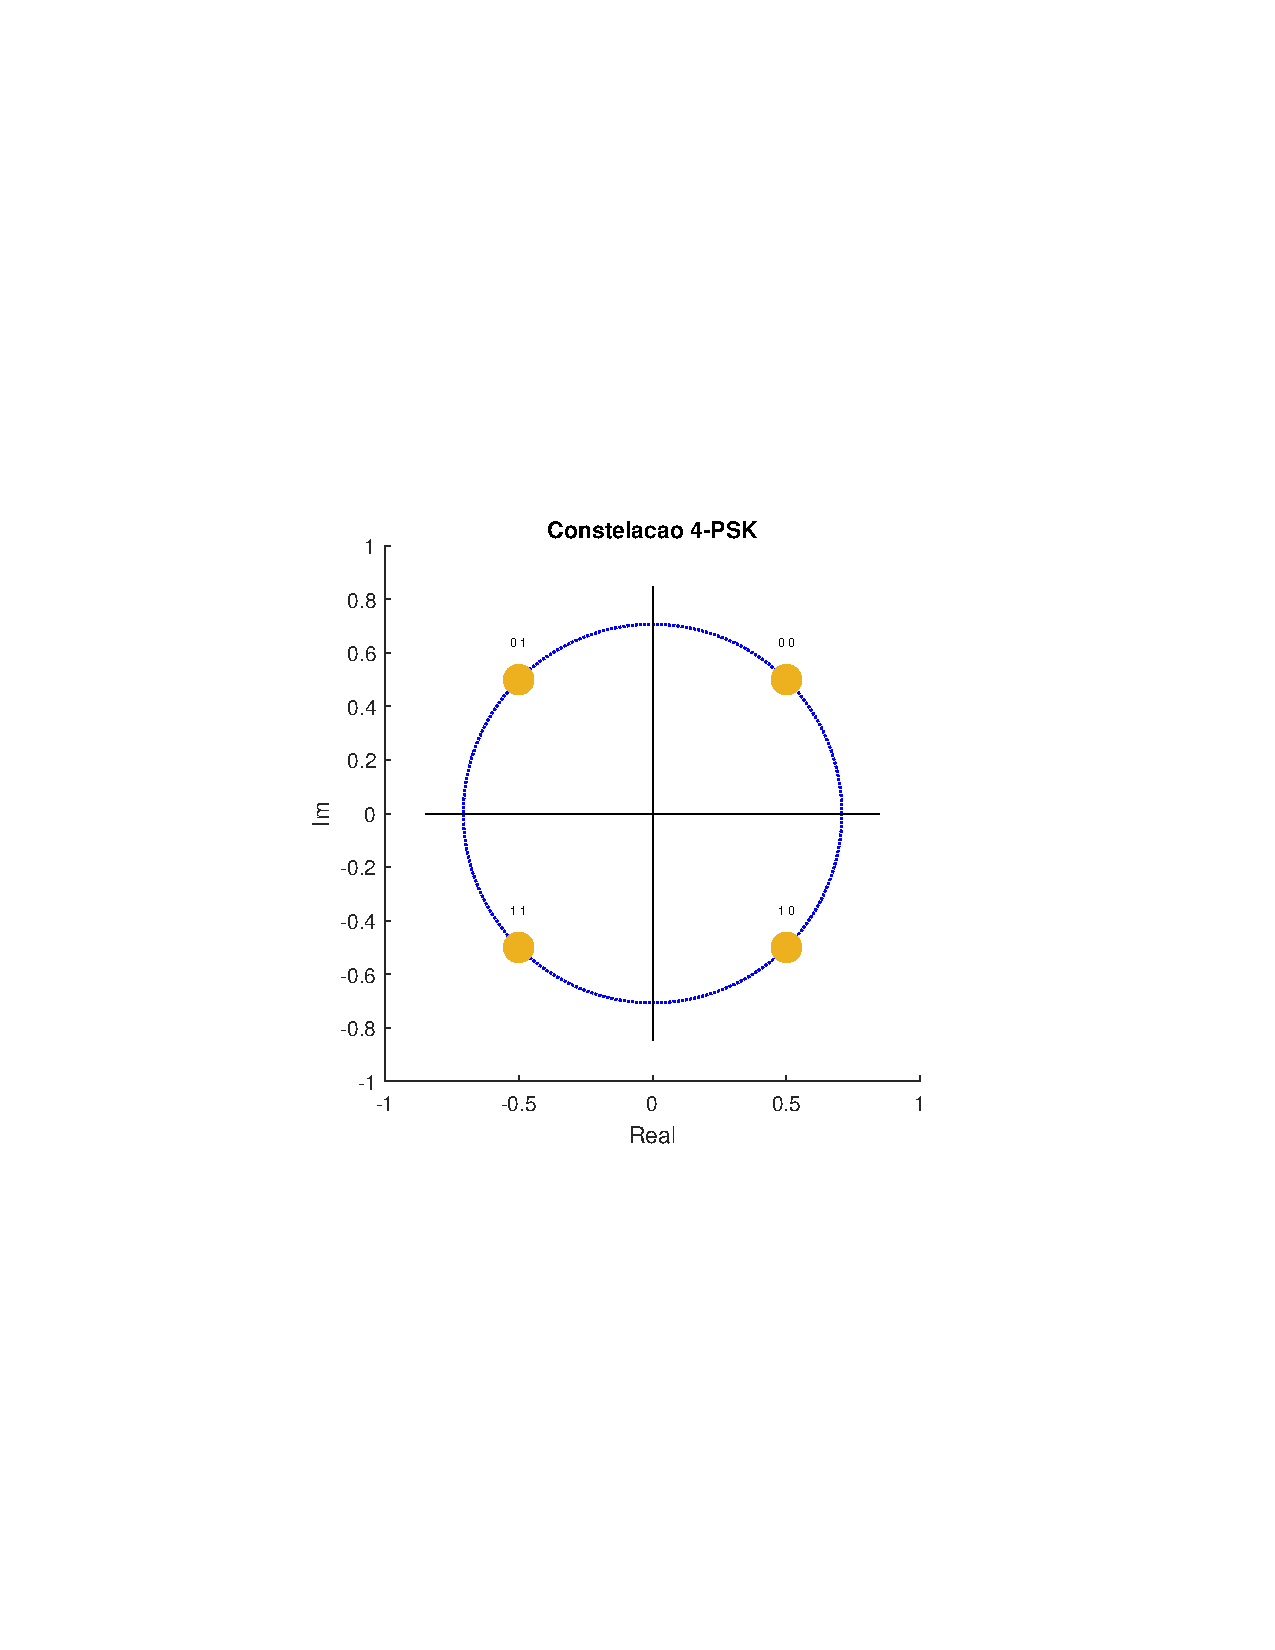
\includegraphics[width=1.0\textwidth,clip=true,trim={1.5cm 8.5cm 1.8cm 8.3cm}]{C:/Users/lukin/Documents/GitHub/Courses-HWs/Sistemas de Comunicacoes Digitais/matlab/problema4/parte1/fig/4_PSK_plot.pdf}
    \caption{Constelação $4$-PSK com codificação de Gray.}
    \label{fig:4_PSK_plot}
\end{figure}

\begin{figure}[!ht]
    \centering
    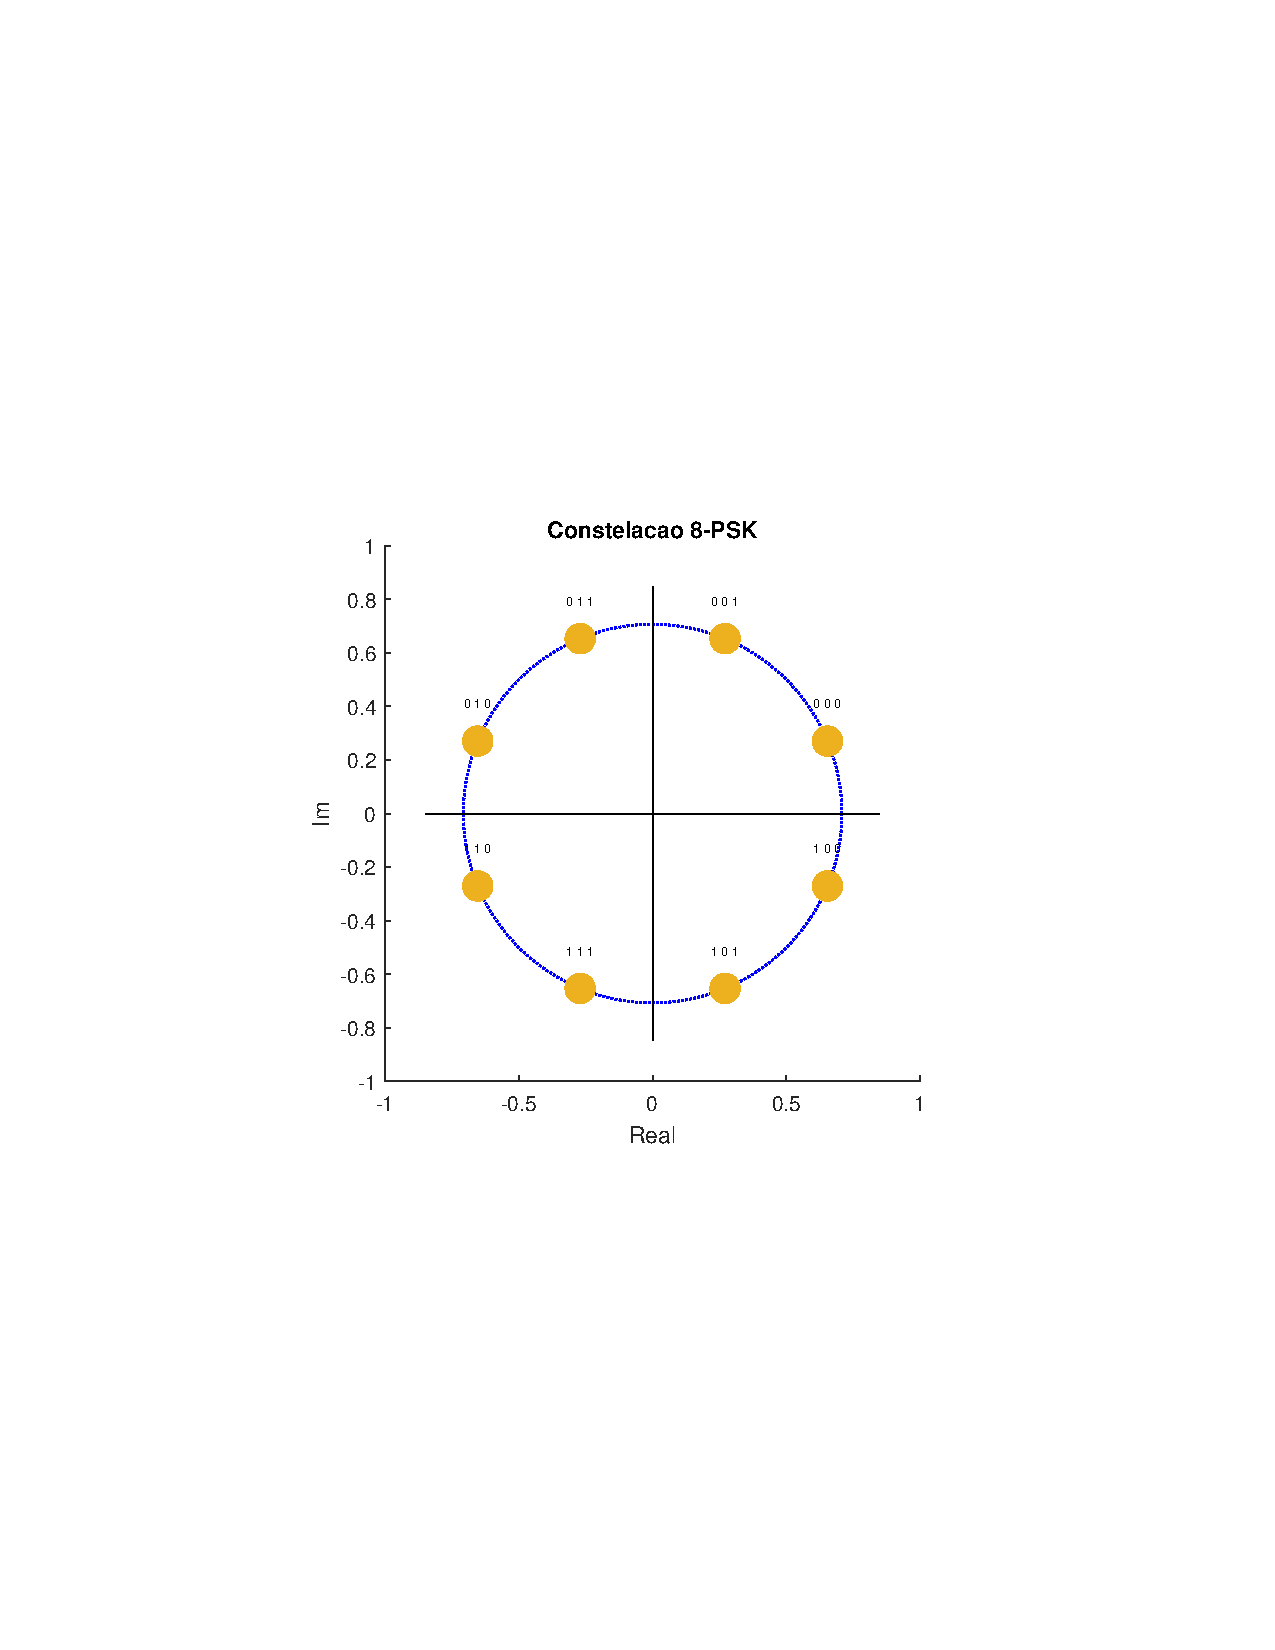
\includegraphics[width=1.0\textwidth,clip=true,trim={1.5cm 8.5cm 1.8cm 8.3cm}]{C:/Users/lukin/Documents/GitHub/Courses-HWs/Sistemas de Comunicacoes Digitais/matlab/problema4/parte1/fig/8_PSK_plot.pdf}
    \caption{Constelação $8$-PSK com codificação de Gray.}
    \label{fig:8_PSK_plot}
\end{figure}

\begin{figure}[!ht]
    \centering
    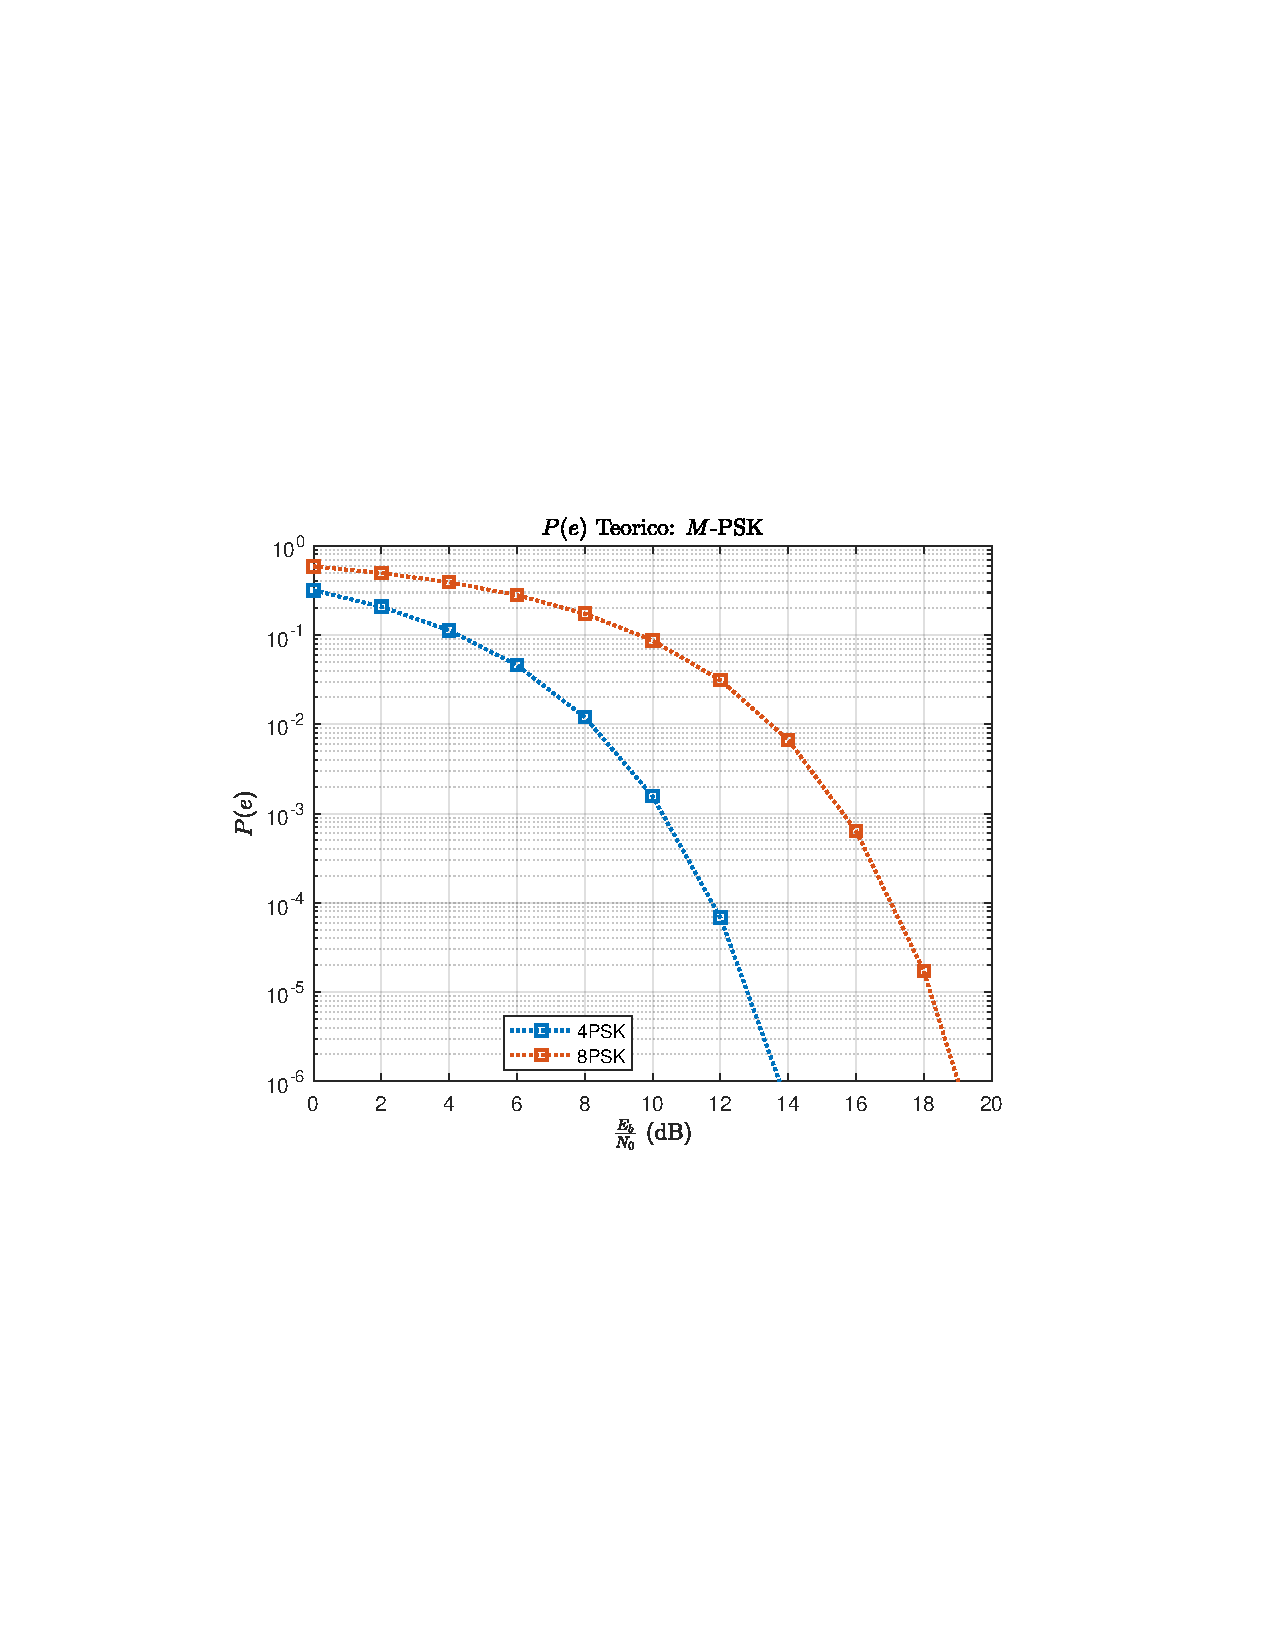
\includegraphics[width=1.0\textwidth,clip=true,trim={1.5cm 8.5cm 1.8cm 8.3cm}]{C:/Users/lukin/Documents/GitHub/Courses-HWs/Sistemas de Comunicacoes Digitais/matlab/problema4/parte2/fig/Erro_Teorico_MPSK.pdf}
    \caption{Probabilidade de erro $(P(e))$ teórico $M$-PSK.}
    \label{fig:Erro_Teorico_MPSK}
\end{figure}


\begin{figure}[!ht]
    \centering
    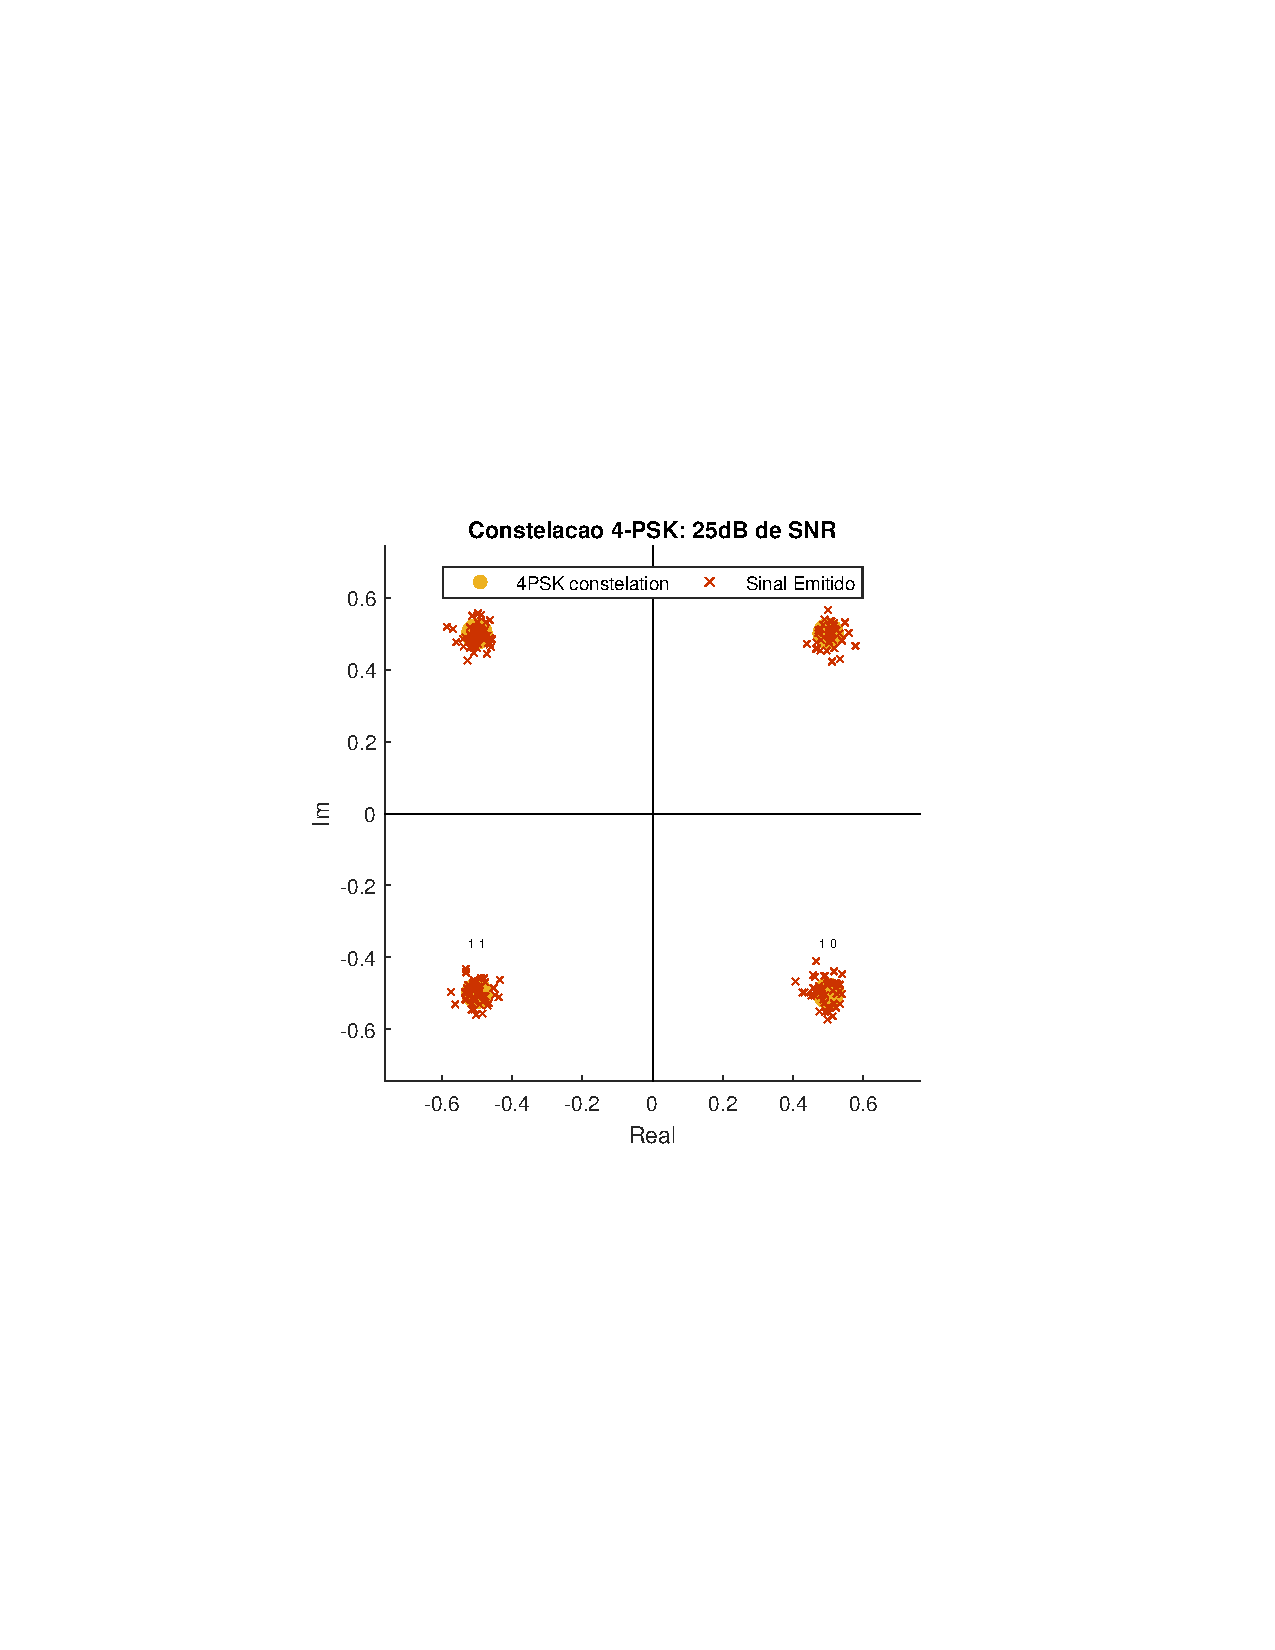
\includegraphics[width=1.0\textwidth,clip=true,trim={1.5cm 8.5cm 1.8cm 8.3cm}]{C:/Users/lukin/Documents/GitHub/Courses-HWs/Sistemas de Comunicacoes Digitais/matlab/problema4/parte3/fig/4PSK_25dB.pdf}
    \caption{Probabilidade de erro $(P(e))$ teórico $M$-PSK.}
    \label{fig:4PSK_25dB}
\end{figure}

\begin{figure}[!ht]
    \centering
    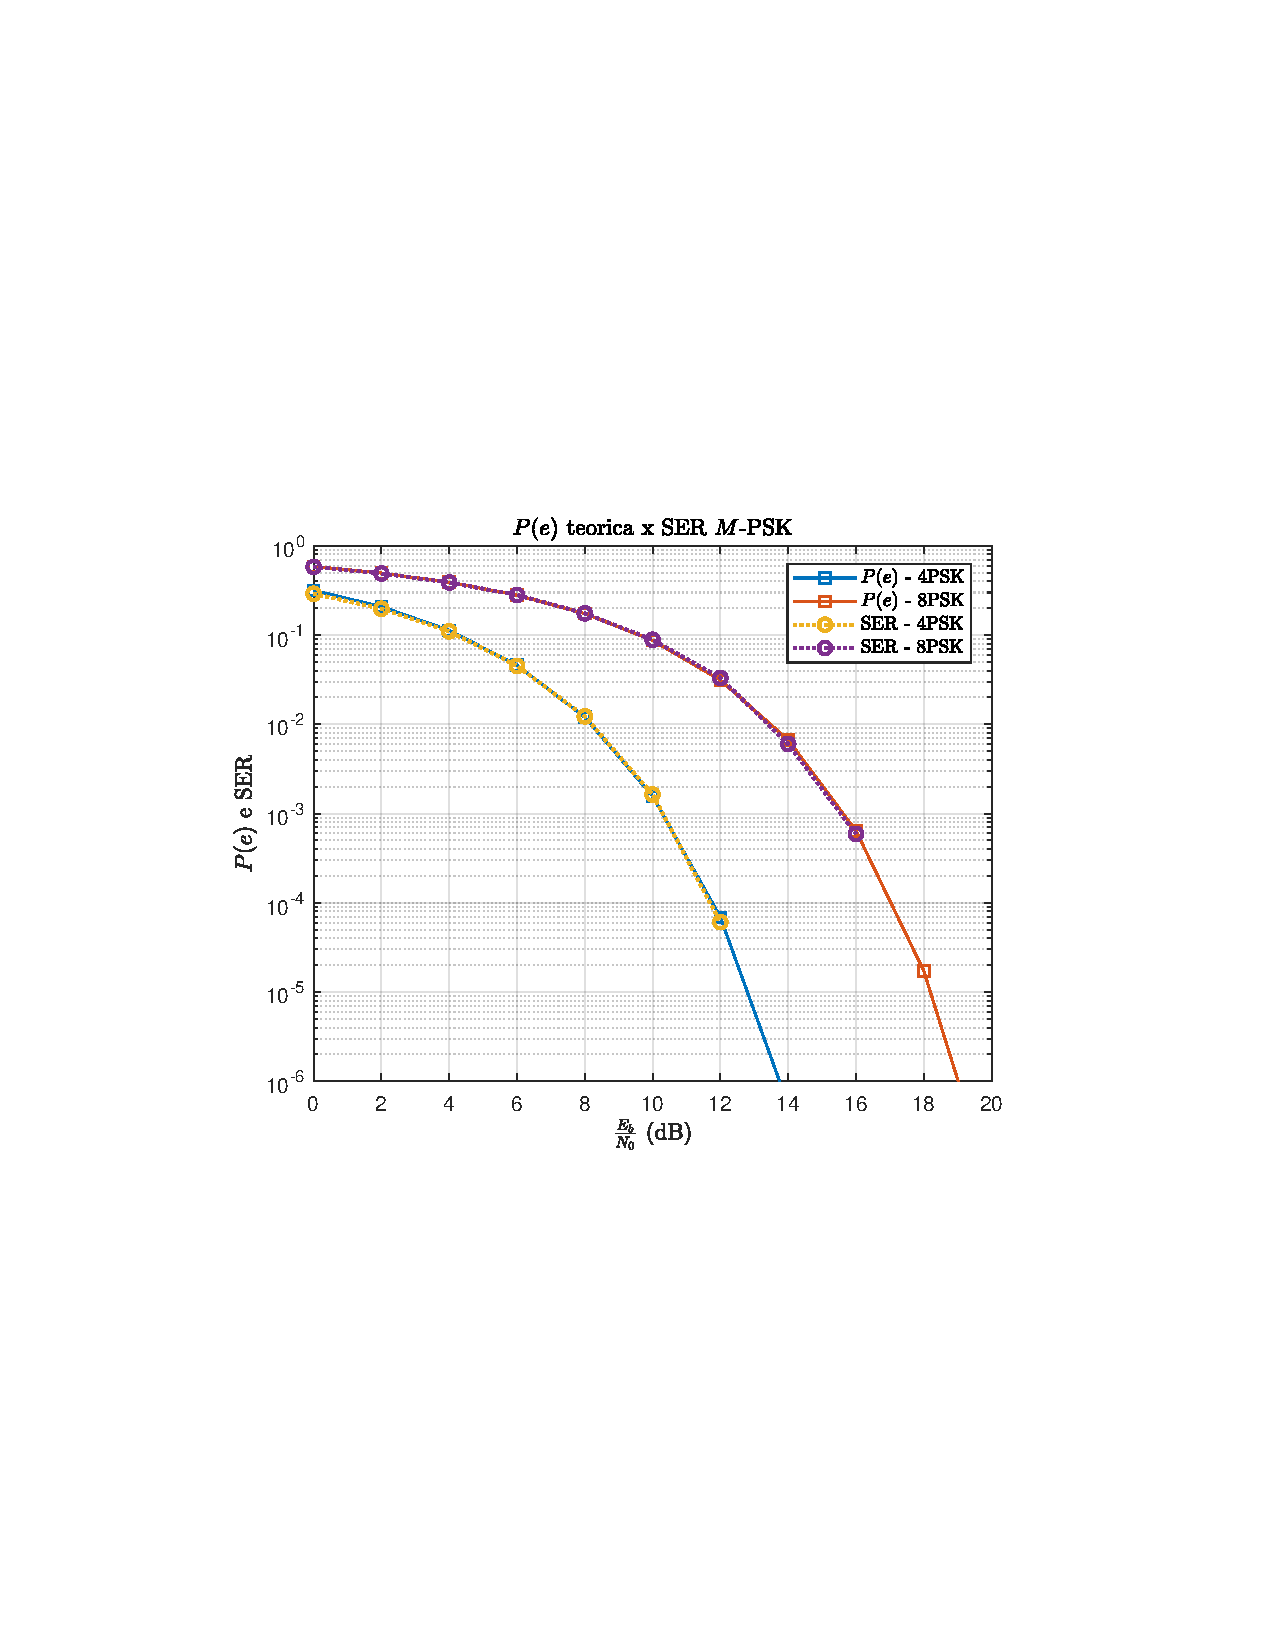
\includegraphics[width=1.0\textwidth,clip=true,trim={1.5cm 8.5cm 1.8cm 8.3cm}]{C:/Users/lukin/Documents/GitHub/Courses-HWs/Sistemas de Comunicacoes Digitais/matlab/problema4/parte3/fig/Erro_teoricaxAWGN_MPSK.pdf}
    \caption{Probabilidade teórica de erro vs. simulação de transmissão $M$-PSK em canal RAGB.}
    \label{fig:Erro_teoricaxAWGN_MPSK}
\end{figure}

